\documentclass{report}

\usepackage[utf8]{inputenc}
\usepackage[T1]{fontenc}
\usepackage[francais]{babel}
%\usepackage{layout}
%\usepackage{geometry}
%\usepackage{setspace}
\usepackage{soul}
\usepackage{ulem}
%\usepackage{eurosym}
%\usepackage{bookman}
%\usepackage{charter}
%\usepackage{newcent}
%\usepackage{lmodern}
%\usepackage{mathpazo}
%\usepackage{mathptmx}
%\usepackage{url}
%\usepackage{verbatim}
%\usepackage{moreverb}
%\usepackage{listings}
%\usepackage{fancyhdr}
\usepackage{wrapfig}
\usepackage{graphicx}
%\usepackage{color}
\usepackage{xcolor}
%\usepackage{colortbl}
\usepackage{amsmath}
\usepackage{amssymb}
\usepackage{mathrsfs}
%\usepackage{asmthm}
%\usepackage{makeidx}
\usepackage{float}


\title{Système autonome pour le traitement et l'exploitation de données GPS}
\author{COUNOT Thibaut et WARTELLE Adrien}
\date{13/06/17}

\begin{document}

\maketitle
\tableofcontents

\chapter{Introduction}
\section{Présenation du groupe}
Nous sommes deux étudiants en branche d'ingénieur à l'UTT :
un en branche A2I 2 (Thibaut) et l'autre en RT 3 (Adrien en filière TMSE). 
Nous avons choisi l'unité d'enseignement IF23 sur la géolocalisation 
principalement parce qu'elle traite 
de problématiques d'informatique embarquée et de modélisation mathématique
pour le traitement de données. Nous sommes en effet intrigués par le
fonctionnement de l'informatique au plus bas niveau, ce sur quoi repose
toutes les technologies modernes.

\section{Cahier des charges}

Dans le cadre de cette unité d'enseigement, nous avons du réaliser
un mini-projet GPS dont l'objectif a été de programmer un SOC (Système
 On Chip) Arduino pour lui permettre de manipuler, d'afficher et 
 d'enregistrer des données satellites. Notre travail s'est décomposé
 en deux parties :
 \begin{itemize}
 \item Programmation du système GPS
 \item Traitement et exploitation des données enregistrées
 \end{itemize}
 En effet, nous avons du programmer un système embarquée
 avec toutes les problématiques d'optimisation que cela implique
  en incorporant des
 fonctionnalités pour l'affichage de l'autonomie, des coordonées
 pour l'enregistrement (horodatage, choix durée d'enregistrrment
 et d'intervalle) et la transmission des données. \\
 De plus, nous avons du effectuer un traitement des données enregistrées
 à l'aide du SOC sur matlab avec
 la transformation de coordonnées dans différents
 repéres (cartésien et local depuis géocentrique). Nous avons testé
 différents protocoles de parcours pour étudier différents phénomènes
 à l'aide d'indicateurs statistiques (moyenne, variance, corrélation). 

\section{Outils et ressources}
La programmation du système GPS a necessité de multiples composants
électroniques : une carte Arduino équipé d'une ATmega328 (8bits, 3.3V,
32ko de Flash et 2ko SRAM), d'une carte SD, d'un écran LCD, d'un boitier
muni de boutons, d'un récepteur GPS et d'interfaces séries pour la 
communication entre les composants. Pour programmer le système GPS, nous
avons utilisé l'environnement de développement d'Arduino qui permet de
compiler du code C/C++ pour un processeur AVR (à l'aide d'avrgcc) et nous
nous sommes servis de Git et d'un fichier TODOLIST
 pour la gestion du projet que l'on peut retrouver
à l'adresse suivante : \\
https://github.com/Adrilord/GogolPS \\

Le traitement des données a nécessité l'intervention du logiciel Matlab
et d'Octave (version libre GNU de matlab)
pour effectuer les calculs rapidement et facilement. Nous avons aussi
utilisé un petit programme pour transformer le format des données brut
en un format KML pour la visualisation.

Nous avons eu de nombreux problèmes avec les composants GPS : 3 problèmes
de déchargement des piles, un problème persistant de carte SD ainsi qu'un
problème d'espace mémoire pour l'enregistrement et la transmission des
données provoqué par le faite que la librairie SD d'Arduino occupe plus
de 50\% des 2ko disponibles en SRAM. Ces multiples problèmes nous
ont fait perdre plusieurs semaines (au moins 3) et nous ont obligés à changer
2 fois de boitiers et à réécrire entièrement 2 fois le programme GPS. 
Ainsi nous n'avons eu au final que quelques jours pour nous occuper
du traitement des données que nous aurions voulu plus approfondir.

\chapter{Programmation du système GPS}
\section{Démarche}
La programmation du système GPS s'est effectué en 4 étapes :
\begin{itemize}
 \item Tests matériels
 \item Tests de modélisation sur ordinateur en C++ puis C
 \item implémentation 1 
 \item implémentation 2 finale
 \end{itemize}
Nous avons effectué de nombreux Tests avant de pouvoir commencer
à implémenter réellement le programme sur Arduino. Nous avons en effet
écrit (et repris) 4 tests matériels (dans Tests/testsMatériel) pour la carte SD
le module GPS, les piles et les boutons. 
Une fois cela effectué nous avons commencé à modéliser notre 
programme en utilisant le patron de conception MVC : Modèle Vue Contrôleur.

Le modèle contient toutes les données du programme qui nous intéressent
avec des données locales pour l'autonomie, les paramètres de temps de parcours
 et toutes les données que l'on peut recevoir depuis le gps. Ce modèle
 est mis à jour régulièrement pour avoir une version actualisée
 (récente) des données que l'on affiche ou enregistre. \\
 
Les vues sont tous simplement les menus à afficher. Ils contiennent
les informations d'affichage pour les cases du LCD et des informations
sur leur configuration et leur configurabilité. Nous avons initialement 
modélisé les menus comme ceci (SW étant les switchs qui permmettent
la transition entre les menus) :

\begin{figure}[H]
	\begin{center}
		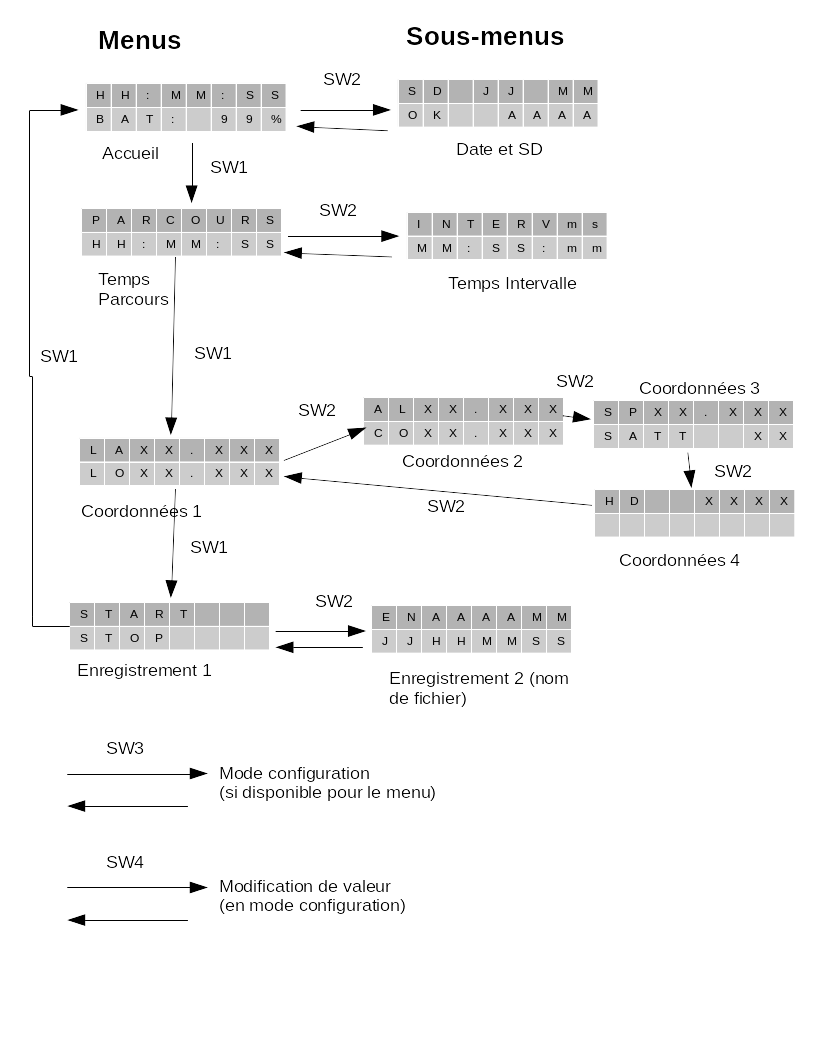
\includegraphics[scale=0.5]{diagrammeCasUtilisation1.png}
	\end{center}
	\caption{Diagramme d'utilisation initial du système}
\end{figure}

Nous n'avons pas implémenté un contrôleur à proprement parler, nous avons
utilisé différents modules à la place qui permettent de manipulé le
modèle et les menus.

Après avoir modélisé notre système, nous l'avons implémenté en C++ (dans Tests/testsCpp) en
utilisant un terminal et le clavier au lieu du système arduino avec lcd
et boutons. Nous nous sommes rapidement rendus compte que la 
programmation orientée objet allait
être lourde et allait imposer une syntaxe difficile tout en nous empêchant
d'optimiser le programme. Nous avons alors réimplémenter cela en C (dans Tests/testC) en
utilisant des structure et des fonctions sur celles-ci. \\
Au moment de transférer le code sur l'arduino, nous avons réalisé que
les fonctions de la librarie standarde de C pour la manipulation des
caractères que nous devions faire n'allait pas être possible (trop de place
prise). Nous avons ainsi reprogrammé des fonctions basiques pour manipuler
les chaines de caractère.

En intégrant la solution dans l'Arduino avec l'implémentation 1
(dans implemArduino), nous nous sommes rendus compte
que, même après avoir optimisé au mieux l'utilisation de la mémoire, il
manquait encore de la mémoire pour pouvoir enregistrer et transférer les
données.

Nous avons alors encore une fois réécrit une implémentation en simplifiant
au maximum le programme : en mettant tout dans le même programme, en
 utilisant uniquement des variables simples (pas de structure), en
 simplifiant au maximum les menus (suppression des sous-menus)
 et ne gardant que les fonctionnalités essentielles.
 (Cette dernière implémentation est dans implemArduino2)
 Nous sommes abouti à ce diagramme :
 
\begin{figure}[H]
	\begin{center}
		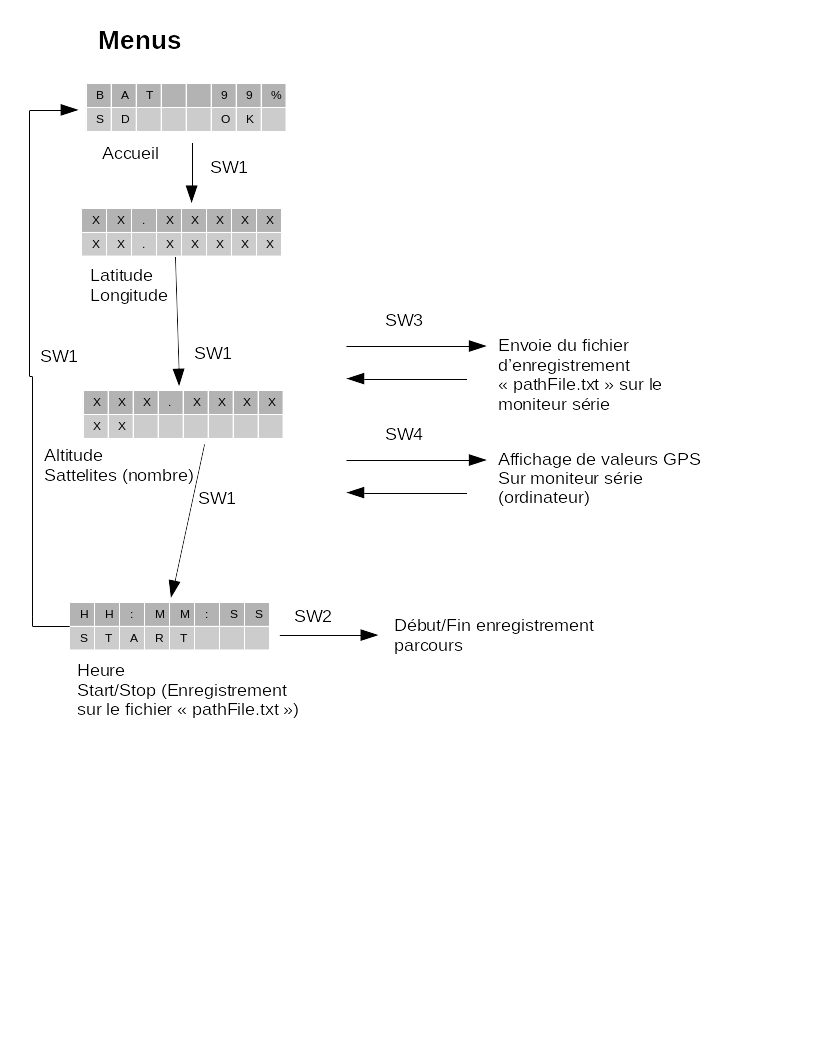
\includegraphics[scale=0.6]{diagrammeCasUtilisation2.png}
	\end{center}
	\caption{Diagramme d'utilisation final du système}
\end{figure}

C'est grâce à cette dernière implémentation que nous avons pu effectuer
les parcours.
 

\section{Modèle MVC et implémentation 1}

La première implémentation sur Arduino est constitué de 6 modules :
\begin{itemize}
\item implemArduino
\item charmanagment
\item datetime
\item iomanagement
\item menu
\item model
\end{itemize}

Le module model contient une structure décrivant le modèle
sous format nombre et une sous format caractères (ASCII). Il contient
aussi des fonctions d'initialisations et mis à jour et de
transformation (format nombre au format caractères). \\
Le module menu contient une structure décrivant un menu avec ses
variables pour la gestion de la configuration (groupe d'id notamment),
et les types de menu auquel il est connecté par SW1 et SW2. Il contient
aussi des fonctions pour l'affichage (pour le lcd), la génération de menu
à partir de son type, la mise à jour du contenu d'un menu et des 
fonctions pour la gestion de la configuration. \\
Le module charmanagement implémente des fonctions simples pour la
manipulation de chaînes de caractères et pour la transformation de
nombres en chaînes de caractères. \\
Le module datetime contient une structure permettant de représenter 
une date avec le temps. On y trouve une fonction d'initialisation.

Le module iomanagement contient une struture pour la configuration
de l'enregistrement d'un parcours. Ce module est partiellement
implémenté car c'est à ce moment que nous nous sommes rendus
compte des problèmes de mémoire. On y trouve des fonctions pour
initialiser la configuration d'enregistrement et des fonctions
pour l'enregistrement des données et des paramètres de temps de parcours.

Finalement le module implemArduino contient le programme principal
que l'on peut résumer par le schéma suivant :

\begin{figure}[H]
	\begin{center}
		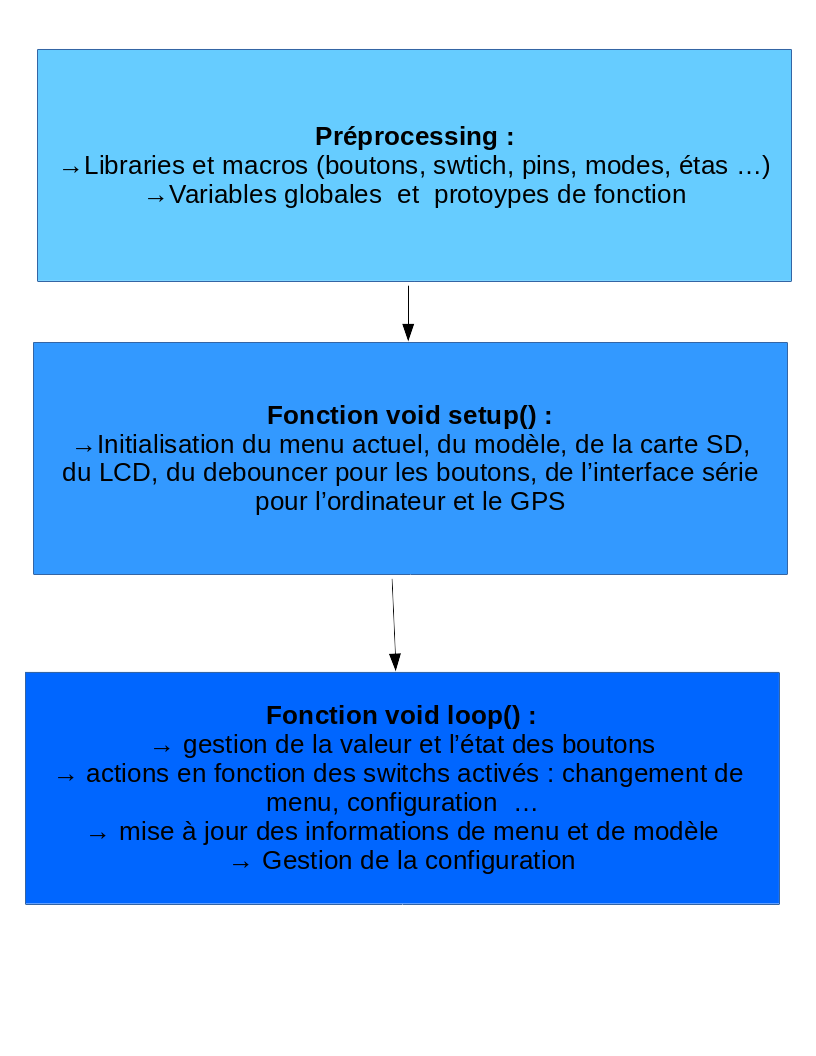
\includegraphics[scale=0.5]{schemaProgramme.png}
	\end{center}
	\caption{Schéma du programme principal}
\end{figure}

Après la fonction loop, on trouve des fonctions pour la gestion
des boutons, pour un délai intelligent pour le GPS qui intègre l'encodage
des données, pour des tests éventuels.

La gestion des boutons consiste à détecter des changements de valeur
des pins, on change alors les états des boutons (attention ce que l'on
appel bouton ici correspond à un signal reçu sur l'arduino et non
à un switch (vraie bouton) du boitier) et en fonction
de la combinaison d'états, on sait quel switch a été activé.

Cette première implémentation permettait de remplir toutes les
fonctionnalités du cahier des charges à l'exception de l'enregistrement.
Nous avons donc mis en place rapidement (il restait de 2 semaines)
une seconde implémentation pour effectuer l'enregistrement de parcours.

\section{Modèle Simple et implémentation 2}

Cette implémentation reprend le programme principal de la première
implémentation tout en intégrant l'affichage et la mise à jour des 
menus et des données de modèle directement dans le code notamment
avec des variables globales simples. On a enlevé la gestion de la
configuration, la gestion des paramètres, simplifié le système de menu.
Nous avons décidé d'utiliser un unique fichier pour l'enregistrement des
parcours ("pathFile.txt") que l'on réécrit à chaque enregistrement. L'intervalle
d'enregistrement est de 5 secondes et on enregistre avec le start/stop
(switch SW3). Il faut donc enregistrer les donnés du parcours précédent
sur ordinateur (grâce à une transmission série) avant de pouvoir
commencer une nouvelle.

Nous avons fait ces choix de simplification pour s'assurer d'avoir
 suffisament de mémoire pour l'enregistrement et donc pour pouvoir 
 rapidement commencer la partie traitement.



\chapter{Traitement et exploitation des données enregistrées}
\section{Protocoles des parcours}
Nous avons effectué trois parcours : un immobile sous un toit (fichier
"enrUno1206"), un mobile autour du parking devant le laboratoire X de
l'UTT en passant sous des arbres (fichier "enrDos1206") et un immobile 
à l'air libre sans grand obstacle devant le foyer étudiant (fichier 
"enrTres1206").
Tous ces enregistrements ont été effectués le 12/06/17 au format "brut"
où les valeurs de GPS sont juste séparés par des virgules sur une ligne
et chaque ligne correspond à un enregistrement (les enregistrements
étant séparés de 5 secondes). Voici les informations (dans l'ordre) 
contenus dans une ligne : \\
longitude,latitude,altitude,nombreDeSatellites,heure,minute,secondes,
hdop \\
L'heure est celle des gps, elle est décalée de 2 heures par rapport
à l'heure locale et elle assez précise.
Tous les fichiers concernant les enregistrements et leur traitements
se trouve dans le dossier Enregistrements.

\section{Visualisation KML}
Le KML (Keyhole Markup Language), est un langage dérivé du formalisme 
XML destiné à organiser les données géographiques pour les logiciels 
de SIG.

Nous avons parser les fichiers au format "brut" en écrivant le programme
matlab writeKML.m, il en résulte trois fichiers pour chaque parcours :
leurs noms commencent par KML et reprennent 
les noms de fichier du format brut.
Le programme ouvre un fichier au format brut, lit les données et 
grâce à la fonction fprintf écrit un fichier au format KML.
 
Un fichier KML commence par un header KML que rien ne peut précéder. 
Ensuite on définit le nom du fichier et une courte description. 
L’utilisateur choisit ensuite un style, on peut choisir un style 
déjà existant en renseignant un id connu, ou créer un style. 
Dans ce fichier on choisit la couleur rouge (501400ff) 
et une largeur de ligne de 10. Si l’on est amené à tracer des polygones, 
on définit aussi un PolyStyle (couleur et opacité).
 
Une fois le style définit on décrit le parcours, 
son nom et sa description. La balise extrude permet d’étendre les lignes 
jusqu’au sol, et tesselate divise le parcours en petits morceaux 
pour suivre la courbure de la terre plus précisément 
(si on choisit d’afficher les données sur Google Earth). 
La balise altitudeMode définit comment la hauteur 
des points est calculée. 
En mode absolute l’altitude est calculée par rapport au niveau de la mer.
 
Enfin on place les coordonnées sous la forme longitude,latitude,altitude 
après la balise coordinates.

Avec l'utilisation du site http://www.gpsvisualizer.com, on a obtenu
les tracées des parcours sur carte (fichier png commencant par parcours) :

\begin{figure}[H]
	\begin{center}
		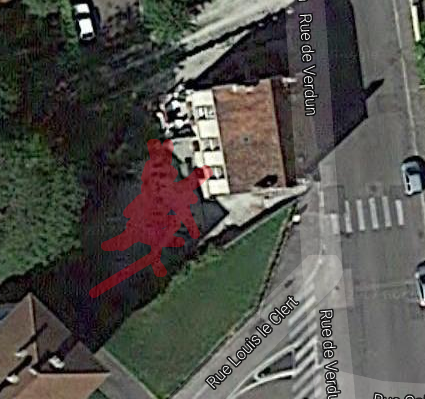
\includegraphics[scale=0.5]{Enregistrements/parcoursEnrUno1206.png}
	\end{center}
	\caption{Tracé du parcours 1}
\end{figure}

\begin{figure}[H]
	\begin{center}
		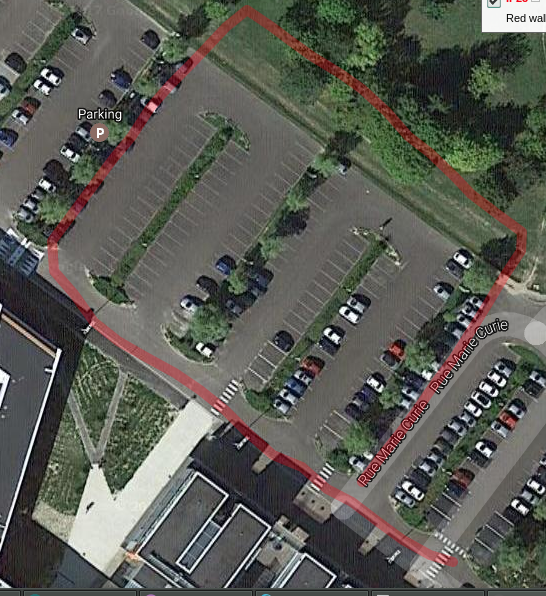
\includegraphics[scale=0.5]{Enregistrements/parcoursEnrDos1206.png}
	\end{center}
	\caption{Tracé du parcours 2}
\end{figure}

\begin{figure}[H]
	\begin{center}
		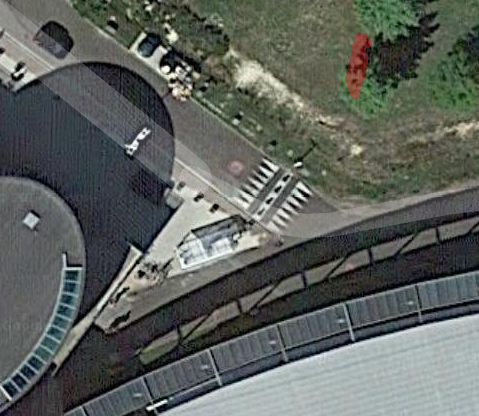
\includegraphics[scale=0.5]{Enregistrements/parcoursEnrTres1206.png}
	\end{center}
	\caption{Tracé du parcours 3}
\end{figure}

On remarque que l'on a finalement une bonne précision
puisque (nous nous souvenant du lieu précis des 
expériences), les positions sont très proches de la
réalité (à quelques mètres). De plus on voit que le
parcours 2 mobile est constitué de lignes droites (comme
effectué lors de l'expérience) et passe aux bons
endroits, les arbres n'ayant pas l'air d'avoir un impact conséquent.
On peut remarquer que les parcours statiques (immobiles) ont quelques
variations autour de la position initiale, il semblerait que le 
parcours 1 soit moins précis que le 3, certainement du à la présence 
d'un toit.


\section{Traitement matlab}
A l'aide du fichier exploitMatlab, nous avons pu facilement exploiter
les données enregistrées. Le programme se décompose en une partie
transformation de données et en une partie affichage d'indicateurs.
Dans la partie transformation de données, on récupère les informations
de localisation (longitude, latitude, altitude) que l'on transforme 
à l'aide des fonctions (dans le même dossier) degDectoRad, ellipToCart,
cartToLocal pour obtenir celles-ci dans un repère local. \\
Le point de référence choisi est : 48.268948 (latitude), 4.068544 (longitude). 
Il s'agit de l'entrée de l'ellipse de l'UTT du côté du
batiment L. \\
La partie affichage d'indicateurs affiche des données résumant
l'enregistrement de manière statistique notamment avec des moyennes et
des écarts.

\section{Résultats}
Pour le premier enregistrement en statique sous un toit nous avons 
(fichier resultatsEnrUno1206) :

\begin{verbatim}
Nombre moyen de sattellites :
 9.8966
Heure GPS de début :
    8
   53
   17
Heure GPS de fin :
    9
   12
   52
Ecart moyen (en secondes) entre 2 enregistrements selon GPS 
(comparé aux 5 secondes réelles) :
 5.0866
Hdop moyen :
 81.983
Distance (en mètres sans prendre en compte l'altitude)
moyenne par rapport au point de référence :
 1769.6
Ecart type de ces distances (en mètres)  :
 4.1929
altitude moyenne (en mètres) :
 140.41
\end{verbatim}

On s'aperçoit que le toit n'a pas eu une grande influence sur le nombre
de satellites puisque que l'on en détecte en moyenne presque 10. On
voit que l'enregistrement a duré presque 15 minutes et que le temps
gps est assez précis puisque l'on a bien un écart moyen d'environ 
5 secondes . Le Hdop moyen donné est très important, pourtant l'écart-type
n'est que de 4.2m. De plus la distance moyenne de 1769.6m,
par rapport au point de
référence de l'UTT semble correcte puisque c'est à mon domicile et que 
j'ai effectué ce tests et j'habite à 2km (environ et pas à vol d'oiseau) 
à pieds de l'UTT.

Pour le second enregistrement mobile dans le parking de l'UTT, on a 
(fichier resultatsEnrDos1206):

\begin{verbatim}
Nombre moyen de sattellites :
 6
Heure GPS de début :
   11
   39
    3
Heure GPS de fin :
   11
   43
   12
Ecart moyen (en secondes) entre 2 enregistrements selon GPS 
(comparé aux 5 secondes réelles) :
 5.0816
Hdop moyen :
 190
Distance (en mètres sans prendre en compte l'altitude) 
moyenne par rapport au point de référence :
 40.430
Ecart type de ces distances (en mètres) :
 26.210
altitude moyenne (en mètres) :
 122.39
Ecart (distance) moyen entre chaque position (en mètres) :
 4.2712
\end{verbatim}
 
L'enregistrement a duré 4min8s.
On a moins de sattelites que lors du premier enregistrement effectué
quelques minutes auparavant, cela montre à quel point les constellations
bougent rapidement. On voit que la distance moyenne par rapport au 
point de référence est un peu basse (c'est plutôt plus proche de 100m
que de 40m). Enfin l'écart moyen entre chaque position semble à peu
près correcte, on s'est bien déplacé de quelques mètres toutes les
5 secondes.

Pour le troisième et dernier enregistrement en statique à l'air libre
devant le foyer étudiant, on obtient (fichier resultatsEnrTres1206) :

\begin{verbatim}
Nombre moyen de sattellites :
 7.6889
Heure GPS de début :
   11
   48
   12
Heure GPS de fin :
   11
   51
   56
Ecart moyen (en secondes) entre 2 enregistrements selon GPS 
(comparé aux 5 secondes réelles) :
 5.0909
Hdop moyen :
 143.11
Distance (en mètres sans prendre en compte l'altitude) 
moyenne par rapport au point de référence :
 30.711
Ecart type de ces distances  (en mètres) :
 1.6313
altitude moyenne (en mètres) :
 122.41
\end{verbatim}

L'enregistrement a duré 3min44s.
Pour cet enregistrement, on observe un ecart-type des distances assez
faible malgré un hdop moyen élevé. Comme précedemment, la distance
moyenne semble légèrement sous-estimée.

Nous avons aussi rajouté l'affichage de la fonction
d'autocorrélation de la distance par rapport au point
de référence grâce à la fonction xcorr (disponible
sous Octave) et nous obtenons :

\begin{figure}[H]
	\begin{center}
		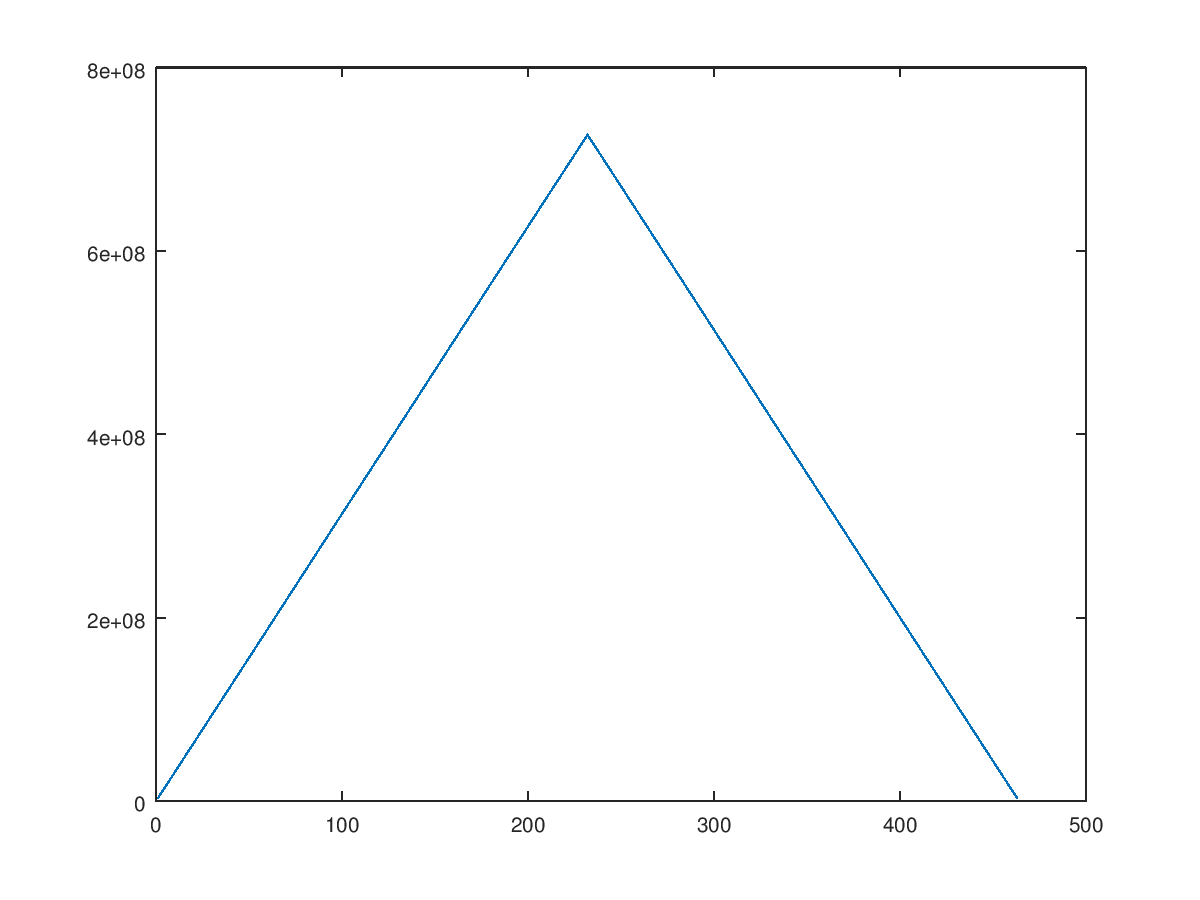
\includegraphics[scale=0.5]{Enregistrements/autocorrelation1.png}
	\end{center}
	\caption{Autocorrélation pour le parcours 1}
\end{figure}

\begin{figure}[H]
	\begin{center}
		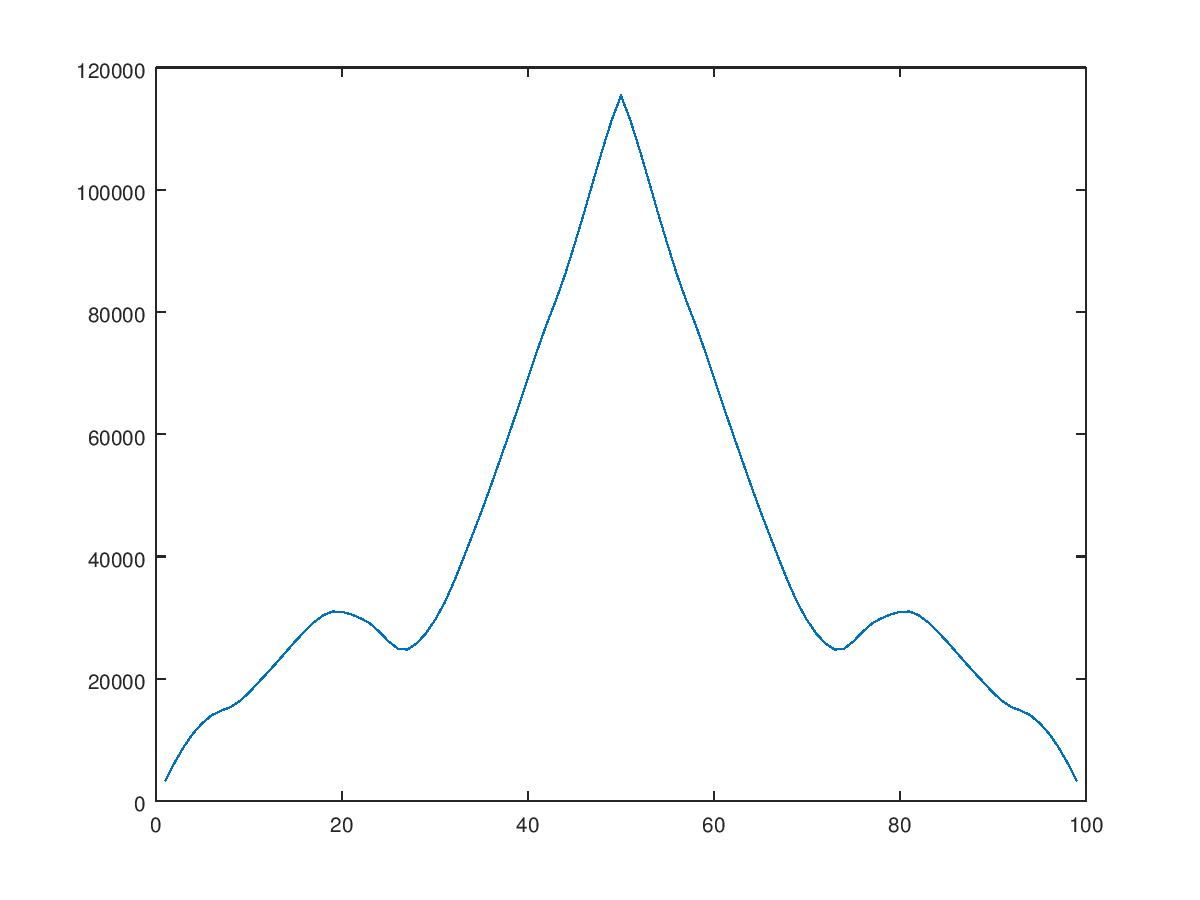
\includegraphics[scale=0.5]{Enregistrements/autocorrelation2.png}
	\end{center}
	\caption{Autocorrélation pour le parcours 2}
\end{figure}

\begin{figure}[H]
	\begin{center}
		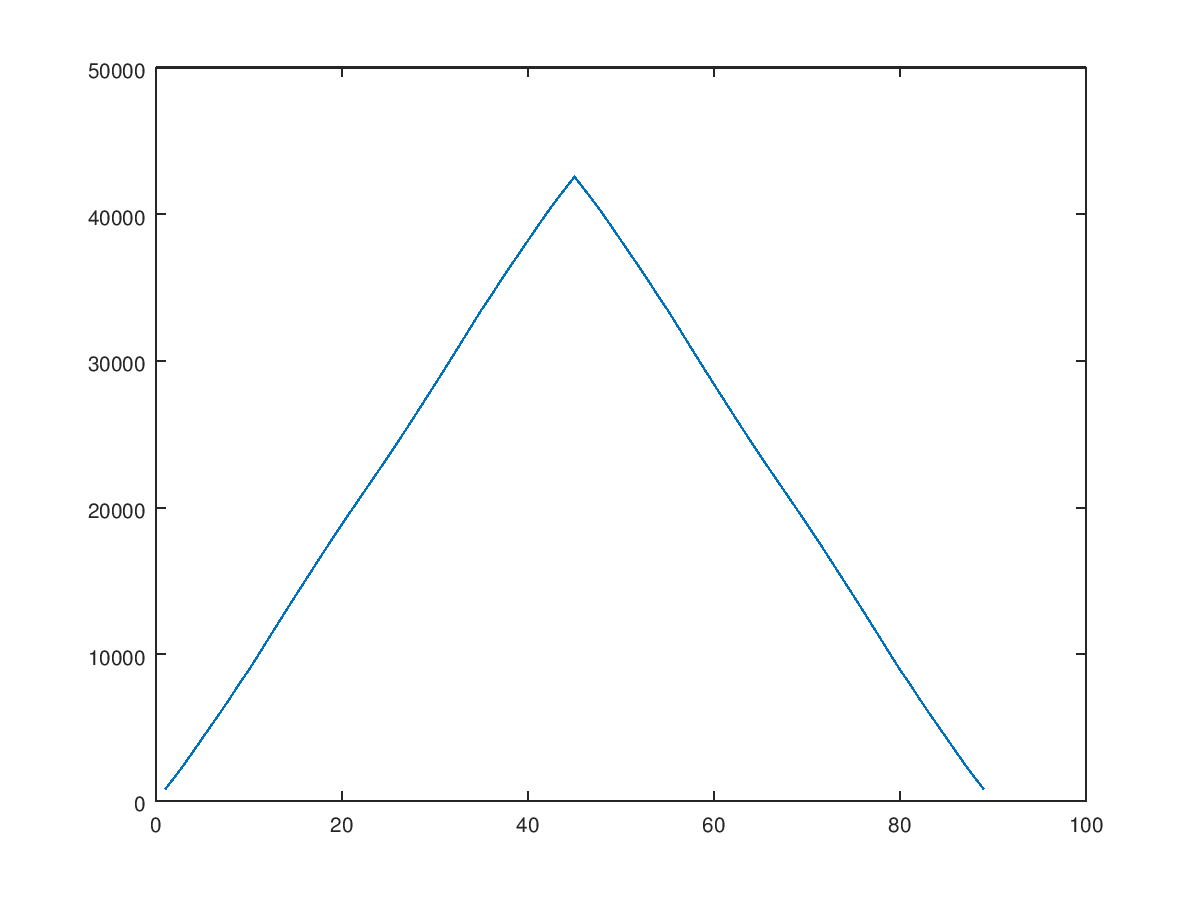
\includegraphics[scale=0.5]{Enregistrements/autocorrelation3.png}
	\end{center}
	\caption{Autocorrélation pour le parcours 3}
\end{figure}

Il manque les légendes d'axes mais l'axe des abscisses
correspond à un nombre d'enregistrements et donc à 
temps si on multiplie par 5 et l'axe des ordonnées
correspond à une distance au carrée ($m^{2}$). De plus
la courbe est mal centré, en effet il aurait fallut mettre le graphique
centré en 0 là où se trouve le maximum de la fonction d'autocorrélation
puisque qu'elle est maximale en 0 (cela aurait nécessité de gérer
le fait que le nombre d'enregistrement est pair ou impair, ce qui aurait
compliqué inutilement le programme).

On reconnait bien la différence entre les parcours
statiques où l'autocorrélation forme un triangle
puisque l'on a un signal rectangle du à la stabilité
de la position et le parcours mobile où l'autocorrélation dimminue 
plus fortement et où un écart de 20 enregistrements (1min40s) provoque
un minimum local.

\chapter{Conclusion}

Nous avons réussi à répondre en grande partie au cahier des charges
imposé malgré les nombreuses difficultés rencontrées. \\
Ce projet nous a permis de développer notre expérience sur la
programmation de systèmes embarquées, sur l'optimisation et la
simplification de programme et sur le traitement de données GPS.

Le SOC Arduino est certainement mal optimisé en terme d'utilisation
d'espace mémoire, en effet l'utilisation de librairies C++  à la place
de librairies C limitent très rapidement nos capacités. Il faudrait soit
utiliser des cartes Arduino plus puissantes, soit utiliser d'autres
types de microcontrôleur, soit programmer en langage C natif avec le
compilateur d'AVR (mais cela demanderait de réécrire beaucoup de fonctions).

Finalement, la programmation d'un système embarqué à faible puissance
provoquera toujours des problèmatiques de choix de modélisation, de 
gestion de la mémoire et de représentations. Néanmoins, nous avons
apprécié le fait d'être confronté à ce genre de problématiques car la
programmation en C à ce bas niveau permet de nous mieux rendre compte
des fonctionnements logiques impliqués dans l'informatique bas niveau.

\end{document}
